\chapter{Eigenvalue and Eigenvector}

\section{Basics}

\begin{definition}
    An eigenvalue of an \(n \times  n\)  matrix A is a nonzero vector x such that \(Ax = \lambda x\) for some scalar \(\lambda \). 
    A scalar \(\lambda \) is called an eigenvalue of A if there is nontrivial solution x of \(Ax = \lambda x\) such an x is called an eigenvector corresponding to \(\lambda \)       
\end{definition}

\begin{remark}
    The eigenvector must be nonzero, but the eigenvalue can be 0.
\end{remark}

Considering the characteristic function \((A - \lambda I)x = 0\), due to the definition, we have an eigenvalue only if we have a nontrivial solution x (which is the eigenvector). To have a nontrivial x, we must have 
%TODO

% \includepdf[pages=-]{}
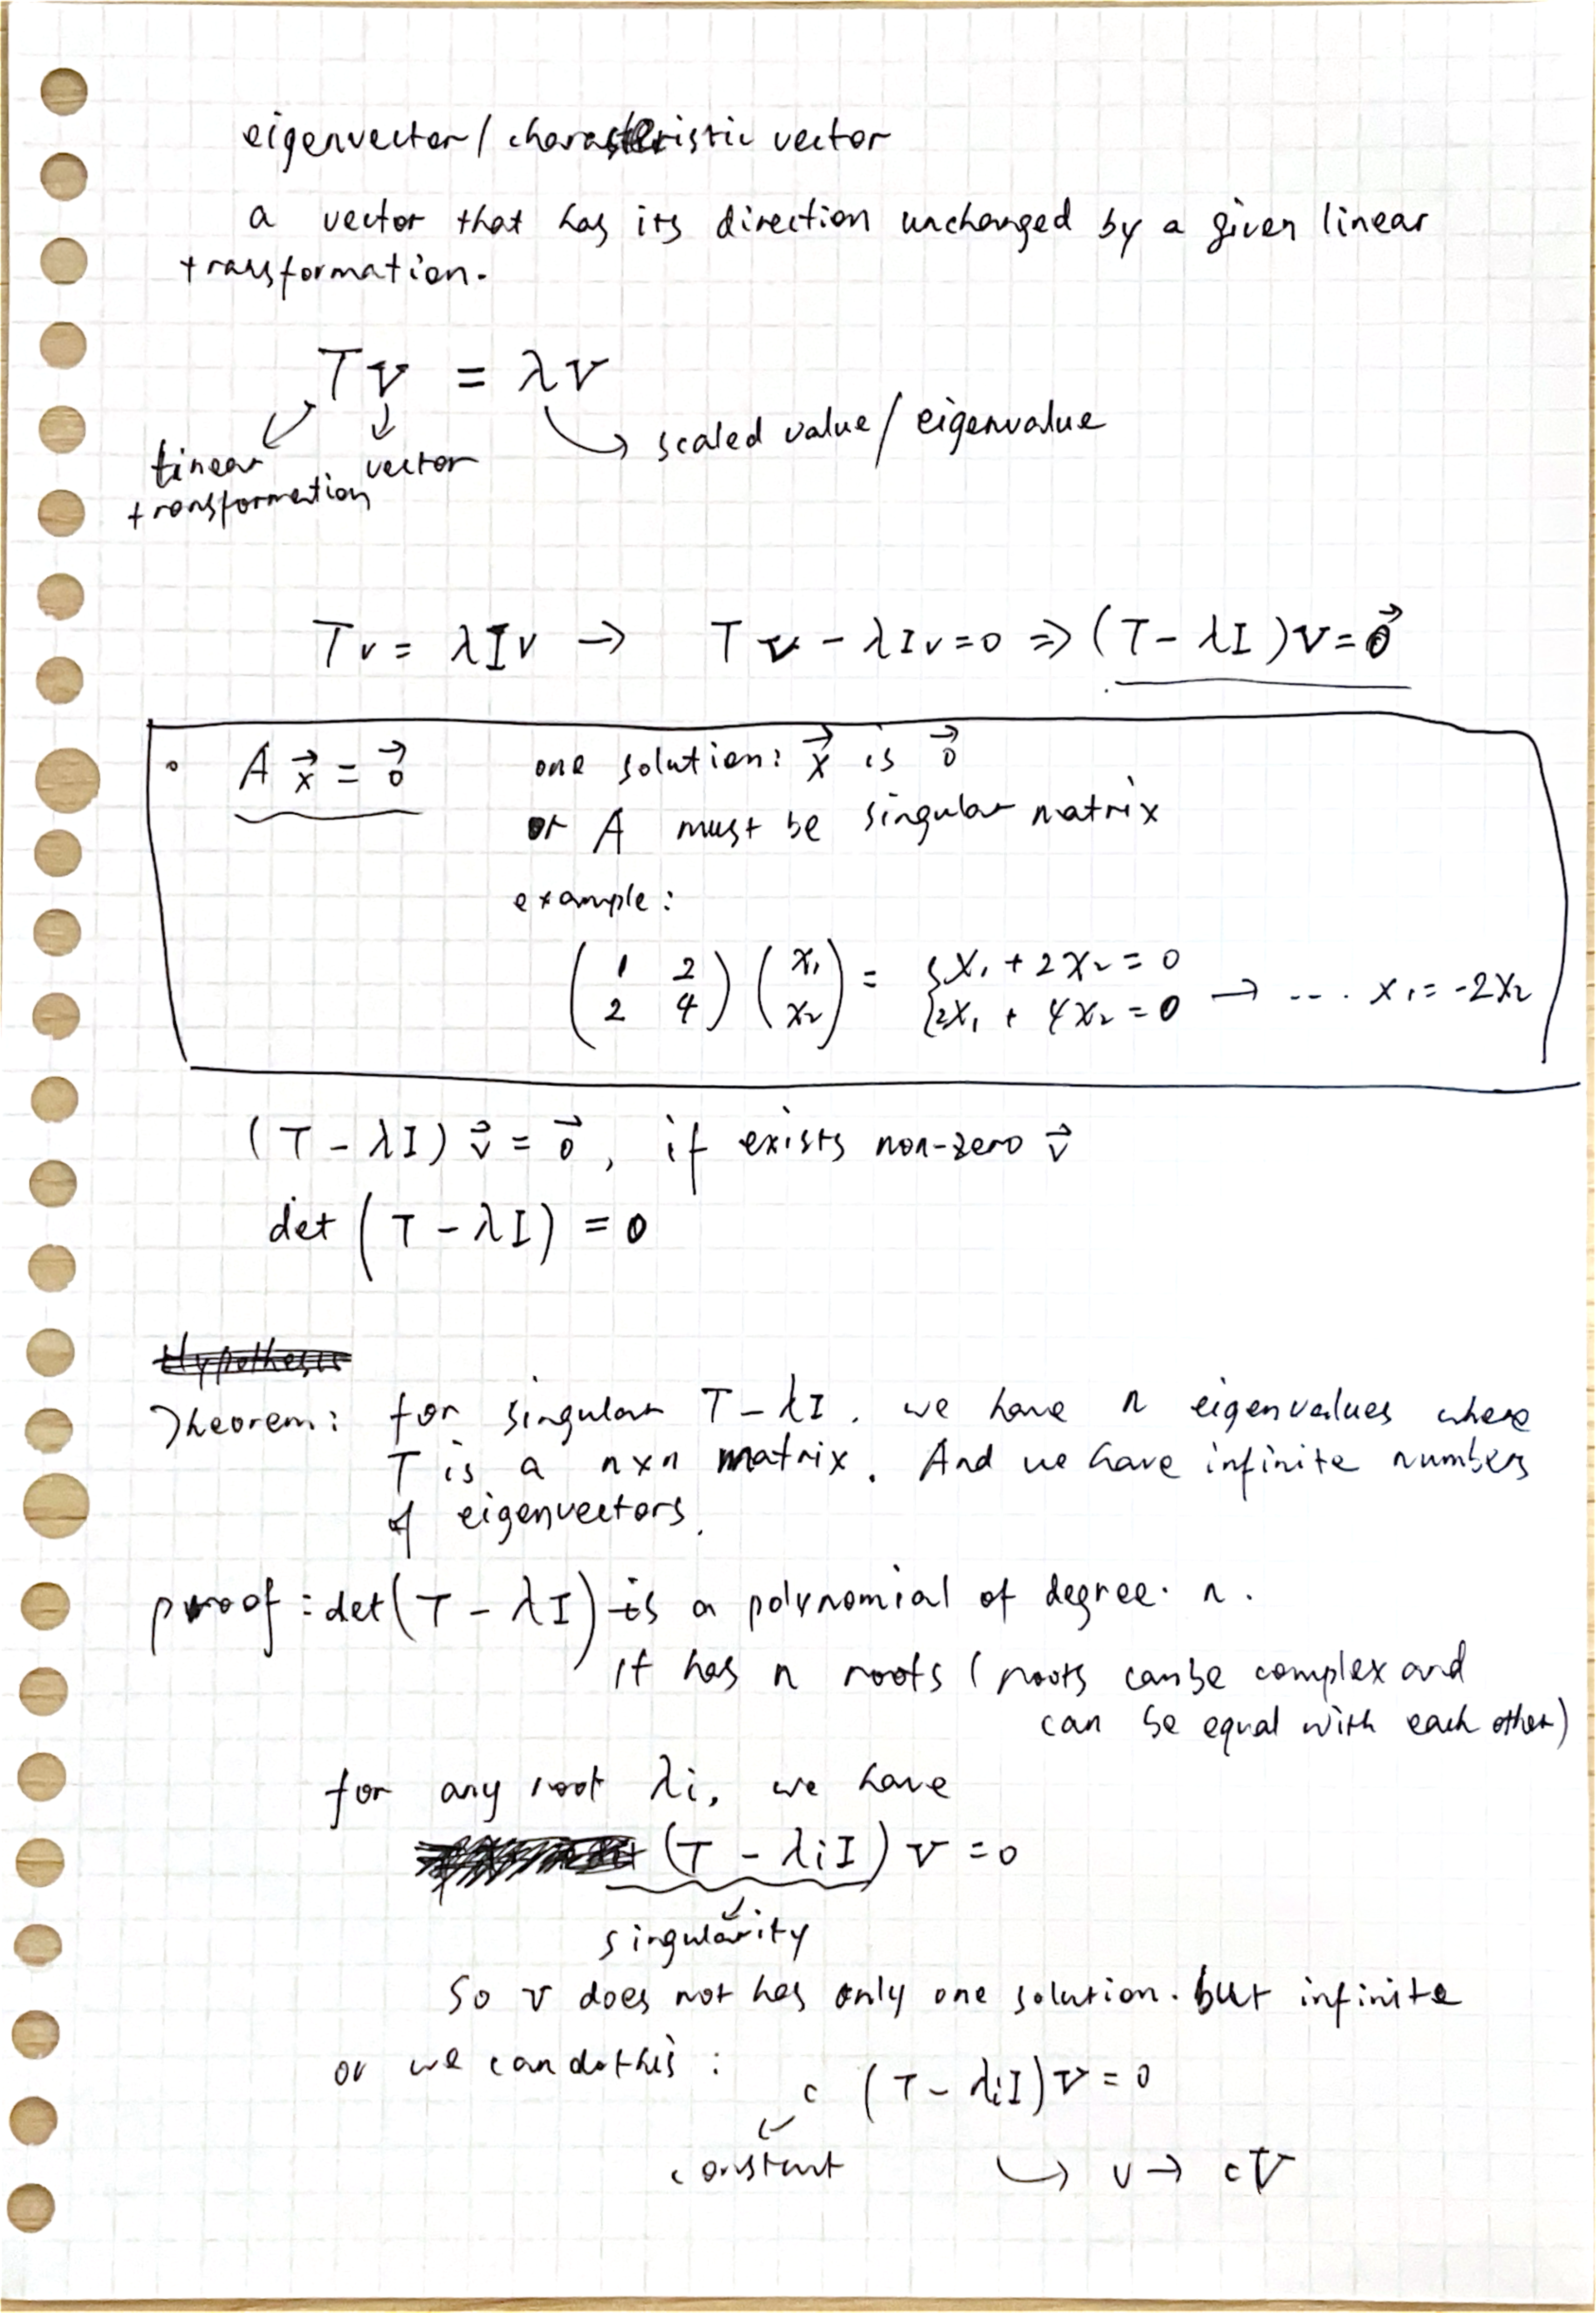
\includepdf[pages=-]{./Draft/eigenvalues.pdf}

\section{Diagonalization}

\begin{definition}[diagonalization]
   An $n  \times n$ matrix $A$ is diagonalizable if it is similar to a diagonal matrix, that is, if there exists an invertible $n \times n$ matrix $C$ and a diagonal matrix $D$ such that:

   $$A = C D C^{-1}$$
\end{definition}

\begin{eg}
    Any diagonal matrix is diagonalizable:  $D = IDI^{-1}$    
\end{eg}

\begin{theorem}[Diagonal Theorem]
    An $n \times n$ matrix A is diagonalizable if and only if $A$ has n linearly independent eigenvectors.

    In this case, $A = CDC^{-1}$ for:

    \[
    C = \begin{pmatrix}
        | & | &  & | \\
        v_1 & v_2 & \cdots & v_n \\
        | & | &  & | 
        \end{pmatrix},
        \qquad
    D = \begin{pmatrix}
        \lambda_1 & 0 & \cdots & 0  \\  
        0 & \lambda_2 & \cdots & 0 \\
        \vdots & \vdots & \ddots & \vdots \\
        0 & 0 & \cdots & \lambda_n 
    \end{pmatrix} 
    \]

    where $v_1, v_2, \dots v_n$  are linearly independent eigenvectors, and $\lambda_1, \lambda_2, \dots \lambda_n$ are the corresponding eignvalues, in the same order.
\end{theorem}

\begin{proof}
   proof 1: If A has n linearly independent eigenvectors - A is diagonalizable     \newline
   (a). $C = (v_1, v_2, \dots, v_n)$ composed of eigenvectors of A is invertible \newline
   (b). 
   \begin{align*}
        AC & = A \begin{pmatrix}
                v_1 & v_2 & \cdots & v_n
                \end{pmatrix} \\
            & = \begin{pmatrix}
                Av_1 & Av_2 & \cdots & Av_n
                \end{pmatrix} \\
            & = \begin{pmatrix}
                \lambda_1v_1 & \lambda_2v_2 & \cdots & \lambda_nv_n
                \end{pmatrix} \\
            & = \begin{pmatrix}
                    v_1 & v_2 & \cdots & v_n
                \end{pmatrix}
                \begin{pmatrix}
                    \lambda_1 & 0 & \cdots & 0  \\  
                    0 & \lambda_2 & \cdots & 0 \\
                    \vdots & \vdots & \ddots & \vdots \\
                    0 & 0 & \cdots & \lambda_n 
                \end{pmatrix} \\
            & = CD
   \end{align*}
   that is, $ACC^{-1} = CDC^{-1} \rightarrow A = CDC^{-1}$

   proof 2: A is diagonalizable - A has n linearly independent eigenvectors \newline
   A is diagonalizable means we can have $A = CDC^{-1}$ where D is a diagonal matrix. Multiply 2 sides of the equation with C, we have AC = CD. We can observe that: \newline
   Left side:
   \begin{align*}
    AC & = A \begin{pmatrix}
                v_1 & v_2 & \cdots & v_n
             \end{pmatrix} \\
       & = \begin{pmatrix}
                Av_1 & Av_2 & \cdots & Av_n
            \end{pmatrix}
   \end{align*}

   Right side:
   \begin{align*}
   CD & =  \begin{pmatrix}
             v_1 & v_2 & \cdots & v_n
           \end{pmatrix}
           \begin{pmatrix}
             \lambda_1 & 0 & \cdots & 0  \\  
             0 & \lambda_2 & \cdots & 0 \\
             \vdots & \vdots & \ddots & \vdots \\
             0 & 0 & \cdots & \lambda_n 
           \end{pmatrix} \\
        & = \begin{pmatrix}
           \lambda_1 v_1 & \lambda_2 v_2 & \cdots & \lambda_n v_n 
        \end{pmatrix}
   \end{align*}

   Which means for any i we have $Av_i = \lambda_i v_i$, so $\lambda_i$ is the eigenvalue and $v_i$  is the eigenvector.
\end{proof}

The above proof has referenced \href{https://leimao.github.io/blog/Matrix-Diagonalization-Theorem/}{this blog article} and \href{https://textbooks.math.gatech.edu/ila/diagonalization.html}{this online textbook from Gatech}.




